%%%%%%%%%%%%%%%%%%%%%%%%%%%%%%%%%%%%%%%%%
% Beamer Presentation
% LaTeX Template
% Version 1.0 (10/11/12)
%
% This template has been downloaded from:
% http://www.LaTeXTemplates.com
%
% License:
% CC BY-NC-SA 3.0 (http://creativecommons.org/licenses/by-nc-sa/3.0/)
%
%%%%%%%%%%%%%%%%%%%%%%%%%%%%%%%%%%%%%%%%%

%----------------------------------------------------------------------------------------
%	PACKAGES AND THEMES
%----------------------------------------------------------------------------------------

\documentclass[xcolor=table]{beamer}

\mode<presentation> {

% The Beamer class comes with a number of default slide themes
% which change the colors and layouts of slides. Below this is a list
% of all the themes, uncomment each in turn to see what they look like.

\usetheme{default}
%\usetheme{AnnArbor}
%\usetheme{Antibes}
%\usetheme{Bergen}
%\usetheme{Berkeley}
%\usetheme{Berlin}
%\usetheme{Boadilla}
%\usetheme{CambridgeUS}
%\usetheme{Copenhagen}
%\usetheme{Darmstadt}
%\usetheme{Dresden}
%\usetheme{Frankfurt}
%\usetheme{Goettingen}
%\usetheme{Hannover}
%\usetheme{Ilmenau}
%\usetheme{JuanLesPins}
%\usetheme{Luebeck}
%\usetheme{Madrid}
%\usetheme{Malmoe}
%\usetheme{Marburg}
%\usetheme{Montpellier}
%\usetheme{PaloAlto}
%\usetheme{Pittsburgh}
%\usetheme{Rochester}
%\usetheme{Singapore}
%\usetheme{Szeged}
%\usetheme{Warsaw}

% As well as themes, the Beamer class has a number of color themes
% for any slide theme. Uncomment each of these in turn to see how it
% changes the colors of your current slide theme.

%\usecolortheme{albatross}
%\usecolortheme{beaver}
%\usecolortheme{beetle}
%\usecolortheme{crane}
%\usecolortheme{dolphin}
%\usecolortheme{dove}
%\usecolortheme{fly}
%\usecolortheme{lily}
%\usecolortheme{orchid}
%\usecolortheme{rose}
%\usecolortheme{seagull}
%\usecolortheme{seahorse}
%\usecolortheme{whale}
%\usecolortheme{wolverine}
%\setbeamertemplate{footline} % To remove the footer line in all slides uncomment this line
\setbeamertemplate{footline}[page number] % To replace the footer line in all slides with a simple slide count uncomment this line

\setbeamertemplate{navigation symbols}{} % To remove the navigation symbols from the bottom of all slides uncomment this line 
}
\usepackage{amsmath} 
\usepackage{graphicx} % Allows including images
\usepackage{booktabs} % Allows the use of \toprule, \midrule and \bottomrule in tables
\usepackage[table]{xcolor}
\usepackage{pgfplots}
\usepackage{tcolorbox}
\pgfplotsset{compat=1.15}
\usepackage{mathrsfs}
\usetikzlibrary{arrows}
\usetikzlibrary{patterns}

\pgfplotsset{ % Define a common style, so we don't repeat ourselves
    MaoYiyi/.style={
        width=0.6\textwidth, % Overall width of the plot
        axis equal image, % Unit vectors for both axes have the same length
        view={0}{90}, % We need to use "3D" plots, but we set the view so we look at them from straight up
        xmin=0, xmax=110, % Axis limits
        ymin=0, ymax=110,
        domain=0:100, y domain=0:100, % Domain over which to evaluate the functions
        xtick={0,20,...,100}, ytick={0,20,...,100}, % Tick marks
        samples=11, % How many arrows?
        cycle list={    % Plot styles
                gray,
                quiver={
                    u={1}, v={f(x)}, % End points of the arrows
                    scale arrows=7.5,
                    every arrow/.append style={
                        -latex % Arrow tip
                    },
                }\\
                red, samples=31, smooth, thick, no markers, domain=0:110\\ % The plot style for the function
        }
    }
}
\usepackage{tikz}
\usepackage{pstricks-add}
\usetikzlibrary{arrows,shapes,positioning,shadows,trees}


\usepackage{tcolorbox}
\usepackage{wrapfig}


\usepackage{hyperref}
\hypersetup{
    colorlinks,
    citecolor=black,
    filecolor=black,
    linkcolor=black,
    urlcolor=black
}
\newcommand{\notimplies}{%
    \mathrel{{\ooalign{\hidewidth$\not\phantom{=}$\hidewidth\cr$\implies$}}}}


\DeclareMathAlphabet\mathzapf{T1}{pzc}{mb}{it}
\usepackage{amsmath,wasysym}
\usepackage{latexsym}

\usepackage{amssymb}
\usepackage{mathrsfs}
\usepackage{bm}
\usepackage{wrapfig}
\usepackage{fancybox}
\bibliographystyle{amsplain}
\usepackage{systeme}
\usepackage{pdfpages}


\usepackage{yfonts}
\usepackage[french]{babel}



\usepackage[T2A]{fontenc}




%\usepackage[style=ieee]{biblatex} %Use if necessary for citation
%\addbibresource{biblatex-examples.bib}
%----------------------------------------------------------------------------------------
%	TITLE PAGE
%----------------------------------------------------------------------------------------

\title[Physique]{Mathématiques II} % The short title appears at the bottom of every slide, the full title is only on the title page

\author{Team Physique} % Your name
\institute[S4S] % Your institution as it will appear on the bottom of every slide, may be shorthand to save space
{
Initiative S4S\\ % Your institution for the title page
\medskip
}
\date{19 septembre 2021} % Date, can be changed to a custom date
\begin{document}

\begin{frame}
\titlepage % Print the title page as the first slide
\end{frame}

\begin{frame}{Approximation et développements limités : Introduction}
\begin{itemize}
    \item Approximer fonction complexe par un polynôme pour simplifier des formules complexes
    \item En physique, principalement utilisé pour $\cos$ et $\sin$
    
\end{itemize}    
\end{frame}
\begin{frame}{Approximations de sinus et cosinus autour de x = 0}

\begin{figure}[ht]

\begin{center}
\definecolor{ccqqqq}{rgb}{0.8,0,0}
\definecolor{qqqqff}{rgb}{0,0,1}
\begin{tikzpicture}[line cap=round,line join=round,>=triangle 45,x=1cm,y=1cm]
\begin{axis}[
x=1cm,y=1cm,
axis lines=middle,
xmin=-2.5400689538405253,
xmax=2.536515566558789,
ymin=-2.111629827594053,
ymax=2.178011872488389,
xtick={-2,-1,...,2},
ytick={-2,-1,...,2},]
\clip(-2.8400689538405253,-2.111629827594053) rectangle (3.136515566558789,2.478011872488389);
\draw[line width=0.8pt,color=qqqqff,smooth,samples=100,domain=-2.8400689538405253:3.136515566558789] plot(\x,{cos(((\x))*180/pi)});
\draw [line width=0.8pt,color=ccqqqq,domain=-2.8400689538405253:3.136515566558789] plot(\x,{(--1-0*\x)/1});
\end{axis}
\end{tikzpicture}
%
\definecolor{ccqqqq}{rgb}{0.8,0,0}
\definecolor{qqqqff}{rgb}{0,0,1}
\begin{tikzpicture}[line cap=round,line join=round,>=triangle 45,x=1cm,y=1cm]
\begin{axis}[
x=1cm,y=1cm,
axis lines=middle,
xmin=-2.5400689538405253,
xmax=2.536515566558789,
ymin=-2.111629827594053,
ymax=2.178011872488389,
xtick={-2,-1,...,2},
ytick={-2,-1,...,2},]
\clip(-2.4558532849474526,-1.8811746892214536) rectangle (2.7186787673463244,2.092541068425681);
\draw[line width=0.8pt,color=qqqqff,smooth,samples=100,domain=-2.4558532849474526:2.7186787673463244] plot(\x,{sin(((\x))*180/pi)});
\draw [line width=0.8pt,color=ccqqqq,domain=-2.4558532849474526:2.7186787673463244] plot(\x,{(-0--1*\x)/1});
\end{axis}
\end{tikzpicture}
\end{center}

\caption{Approximation linéaire du cosinus (à gauche) et du sinus (à droite) autour de $0$}
    \label{fig:dl}
\end{figure}

\begin{tcolorbox}
    \begin{itemize}
        \item $\cos(x) \approx 1$
        \item $\sin(x) \approx x$
    \end{itemize}
\end{tcolorbox}

\end{frame}

\begin{frame}{Développement limités et formule de Taylor}
    \begin{itemize}
        \item Approximation linéaire autour de x = a:
    \[ f(x) \approx f(a) + f'(x)(x-a) \]
    
        \item Formule de Taylor: \[f(x) = \sum_{k=0}^{n} \frac{f^{(k)}(a)}{k!}(x-a)^k + R_n(x) \]
    \end{itemize}
    
\end{frame}

\begin{frame}{Approximation et développements limités : }
    

%Dessin de l'approximation
\begin{figure}
    
    
\definecolor{ffqqqq}{rgb}{1,0,0}
\definecolor{qqqqff}{rgb}{0,0,1}
\begin{center}

\begin{tikzpicture}[line cap=round,line join=round,>=triangle 45,x=1cm,y=1cm,scale=0.5
]
\begin{axis}[
x=2cm,y=1cm,
axis lines=middle,
xmin=-3.780437787628234,
xmax=4.220977016145955,
ymin=-3.0784578863074157,
ymax=3.0661263520169277,
xtick={-3.5,-2.5,...,3.5},
ytick={-3,-2,...,3},]
\clip(-3.780437787628234,-3.0784578863074157) rectangle (4.220977016145955,3.0661263520169277);

\draw[line width=0.8pt,color=red,smooth,samples=100,domain=-3.780437787628234:4.220977016145955] plot(\x,{(\x)});
\draw[line width=0.8pt,color=green,smooth,samples=100,domain=-5.1874758166367645:5.462407287186683] plot(\x,{(\x)-(\x)^(3)/6});
\draw[line width=0.8pt,color=yellow,smooth,samples=100,domain=-5.660273317658524:6.05459809654727] plot(\x,{(\x)-(\x)^(3)/6+(\x)^(5)/120});
\draw[line width=1pt,color=blue,smooth,samples=100,domain=-3.780437787628234:4.220977016145955] plot(\x,{sin(((\x))*180/pi)});
\begin{scriptsize}

\end{scriptsize}
\end{axis}
\end{tikzpicture}
\end{center}


\caption{Approximation de la fonction sinus avec de polynômes de Taylor de différents degré}
    \label{fig:my_label}
\end{figure}
\begin{itemize}
    \item En rouge, l'approximation linéaire $f(x) = x$, qu'on a déjà vu
    \item En vert, l'approximation de degré 3 $g(x) = x - \frac{x^3}{6}$
    \item En jaune, l'approximation de degré 5 $h(x) = x - \frac{x^3}{6} + \frac{x^5}{120}$
\end{itemize}  
\end{frame}
\begin{frame}{Equations différentielles :}
\begin{itemize}
    
    \item  Equation où l'inconnue est une fonction et une plusieurs de ses dérivées sont présentes
    \item Utilisé pour la modélisation de systèmes physiques ou biologiques qui évoluent
    \item Croissance population, coronavirus, diffusion d'un liquide, etc
    \end{itemize}
    \begin{figure}
        \centering
        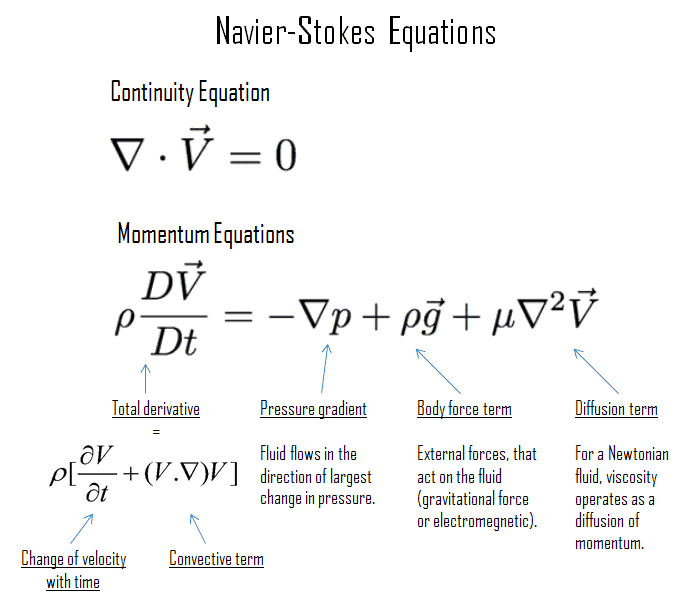
\includegraphics[scale = 0.2]{Images/Navier-Stokes-Equations-definition (1).png}
        %\caption{Caption}
        \label{fig:lab}
    \end{figure}
    
\end{frame}
\begin{frame}{Equations différentielles : Application }
\begin{tcolorbox}[Title=Enoncé]
    On considère un réservoir d'eau cylindrique, de hauteur $h$ et de rayon $R$. On remplit le réservoir d'un liquide et on se rend alors compte que le fond du réservoir est troué par un trou de rayon $r$, avec $r << R$. En tant que physicien, au lieu de prendre du scotch pour boucher le trou, vous décidez d'analyser la situation (oui oui, c'est parfaitement le bon moment). \\
Soit $y(t)$ une fonction qui représente le hauteur du liquide dans le réservoir au temps t. On suppose que le liquide quitte le réservoir à une vitesse $2\sqrt{gy}$. La question est donc la suivante: Si le réservoir est plein au temps t = 0, combien de temps faut-il pour qu'il se vide ?
\end{tcolorbox}

    
\end{frame}

\begin{frame}{Exercices : dérivée}
     Lors de la Welcome Party, vous participez à une course relais avec votre groupe de coaching. Votre camarade a pris du retard que vous devez rattraper. Vous savez que la vitesse nécessaire en fonction du temps s’écrit ainsi : \[v(t) = a e^{-t/b}-bc \]
où $t$ le temps et $a,b$ et $c$ des constantes. Trouver $\Dot{v}$ (la dérivée de la vitesse par rapport au temps).

    \begin{itemize}
        \item $\Dot{v} = -ab e^{-\frac{t}{b}}-bct +d$
        \item $\Dot{v} =- (\frac{a}{b})e^{-\frac{t}{b}}$ %bonne reponse
        \item $\Dot{v} =- (\frac{a}{b})e^{-\frac{t}{b}}-bc$
        \item $\Dot{v} = (\frac{a}{b})e^{-\frac{t}{b}}$ 
    \end{itemize}
\end{frame}

\begin{frame}{Exercice : Primitive}
    Maintenant que vous avez trouvé l'accélération, trouver l'équation horaire (la formule de la position) associé à cette vitesse. Rappel:
     \[v(t) = a e^{-t/b}-bc \]
    
    \begin{itemize}
        \item  $x(t) = -abe^{-\frac{t}{b}}-bct +d$
        \item $x(t) = -abe^{-\frac{t}{b}}-bct $
        \item $x(t) = abe^{-\frac{t}{b}}-bct +d$
        \item $x(t) = -abe^{-\frac{t}{b}}-bc +d$

    \end{itemize}
\end{frame}

\begin{frame}{Exercice: fonction et variable}
Soit $\phi(t)$ une fonction qui représente l'angle $\phi$ d'une point par rapport au temps. Que vaut l'expression suivante:
    \[ \frac{d}{dt}(sin^2(\Dot{\phi}))\] %forme (f(g(h(t)))
    \begin{itemize}
        \item $\Ddot{\phi} \; \sin{2 \Dot{\phi}}$ %réponse correcte (je crois lel)
        \item $\sin{(2 \Dot{\phi})}$ %oubli de la seconde dérivée interne
        \item $ 2\Ddot{\phi} \; \cos{\Dot{\phi}} $ %oublie de la première derivee interne
        \item $2 \Ddot{\phi} \; \sin{\Dot{\phi}}$
    \end{itemize}
    
\end{frame}

\begin{frame}{Exercices: produit scalaire}
    Soient 2 vecteurs u et v dans un  repère cartésien direct (O,x,y,z) : $\Vec{u} = (b,0,a)$ et $\Vec{v} = (bsin(c),-bcosc,a)$ (avec a,b et c des constantes). Que doivent valoir a,b,c pour que $\Vec{u} \cdot \Vec{v} =0 $ ? 
    \begin{itemize}
        \item a=0, b=1, c=$\pi$  %bonne
        \item peu importe les valeurs de a,b,c
        \item a=0, b=5, c=$\dfrac{\pi}{2}$
        \item a=0, b=1, c=\dfrac{\pi}{2}
        
    \end{itemize}
\end{frame}

\begin{frame}{Exercices: produit vectoriel}
Que vaut $\Vec{a} \times \Vec{a}$ ?
    \begin{itemize}
        \item $ \lVert \Vec{a} \rVert ^2$
        \item Cette opération n'est pas définie
        \item Cela dépend de la norme de $\Vec{a}$
        \item $\Vec{0}$
    \end{itemize}
    
\end{frame}
\begin{frame}{Exercices: produit vectoriel}
    

Que vaut $\Vec{b} \times \Vec{a}$
    \begin{itemize}
        \item $\Vec{0}$
        \item $- \Vec{a} \times \Vec{b}$
        \item $\Vec{a} \times \Vec{b}$
        \item Cela dépend
    \end{itemize}
    \end{frame}
    
    \begin{frame}{Exercices: projections}
     Dans cette situation, projetez le vecteur poids $\Vec{P}$ sur les axes $x$ et $y$:
    \begin{figure}[H]
        \centering
        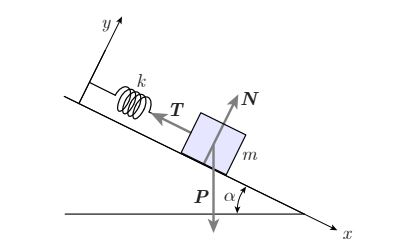
\includegraphics[scale=0.5]{Images/projections_kahoot.JPG}
        %\caption{Caption}
        \label{fig:proj_k}
    \end{figure}
    \begin{itemize}
        \item $\textbf{P} = P\;(\sin{\alpha} \; \hat{\textbf{x}} - \cos{\alpha} \; \hat{\textbf{y}})$ %réponse correcte
        \item $\textbf{P} = P\;(\cos{\alpha} \; \hat{\textbf{x}} + \sin{\alpha} \; \hat{\textbf{y}})$
        \item $\textbf{P} = P\;(\cos{\alpha} \; \hat{\textbf{x}} - \sin{\alpha} \; \hat{\textbf{y}})$
        \item $\textbf{P} = P\;(\sin{\alpha} \; \hat{\textbf{x}} + \cos{\alpha} \; \hat{\textbf{y}})$
    \end{itemize}
        
    \end{frame}
    
    \begin{frame}{Exercice: approximation linéaire}
Trouver une approximation linéaire de tan(x) autour de x = 0:
    \begin{itemize}
        \item $f(x) = \frac{1}{x}$
        \item $f(x) = 1 + x$
        \item $f(x) = x$ %bonne réponse
        \item $f(x) = x + \frac{x^3}{3}$
    \end{itemize}
    
\end{frame}

\begin{frame}{Exercice: Equation différentielle}
    Pour trouver les constantes d'intégrations d'une équation différentielle, on utilise:
    \begin{itemize}
        \item Cela va dépendre du type d'équations différentielles
        \item Les conditions initiales
        \item Cela importe peu, on peut leur donner une valeur arbitraire (souvent 0)
        \item Les valeurs de $f'(0)$ et $f''(0)$
    \end{itemize}
\end{frame}

\begin{frame}{Exercice: Équation différentielle}
Que vaut la solution de l'équation linéaire \[ y'(x) = 2x \cdot y(x)\] avec la condition initial $y(0) = 2$
\begin{itemize}
        \item $y(x) = 2e^{2x}$
        \item $y(x) = e^{x^2}$
        \item $y(x) = 2e^{x^2}$
        \item $y(x) = e^{2x}$
    \end{itemize}
    
\end{frame}
\end{document}